\chapter{مدیریت MySQL از طریق مرورگر}
در فصل قبل به تنظیم مای‌اس‌کیوال و پی‌اچ‌پی پرداختیم. در تنظیمات انجام شده به راحتی قادر خواهید بود تا اکثر کدهای نوشته شده با زبان پی‌اچ‌پی را که به پایگاه داده مای‌اس‌کیوال متصل اند را اجرا کنید. سرور بالا حالا تقریبا به یک سرور کامل مبدل گشته است که علاوه بر امکان ارسال پیغام به وسیله رایانامه قادر به اتصال به پایگاه داده  اسکیو‌لایت نیز هست. در این قسمت در ابتدا یک پیشخوان برای سندباکس ایجاد خواهیم کرد که با مراجعه به آن تمامی نرم‌افزارهای مبتنی بر وب و دیگر موارد دلخواه در آن قابل دسترسی باشند. در این مطلب قصد نداریم به آموزش زبان پی‌اچ‌پی بپردازیم، بنابراین به آموزش کدهای نوشته شده در این مقاله نیازی نیست و فقط کافی است کدهای نوشته شده را در سرور خود قرار دهید تا به راحتی بتوانید به قسمت‌های مختلف سرور خود دسترسی داشته باشید.
\begin{figure}
    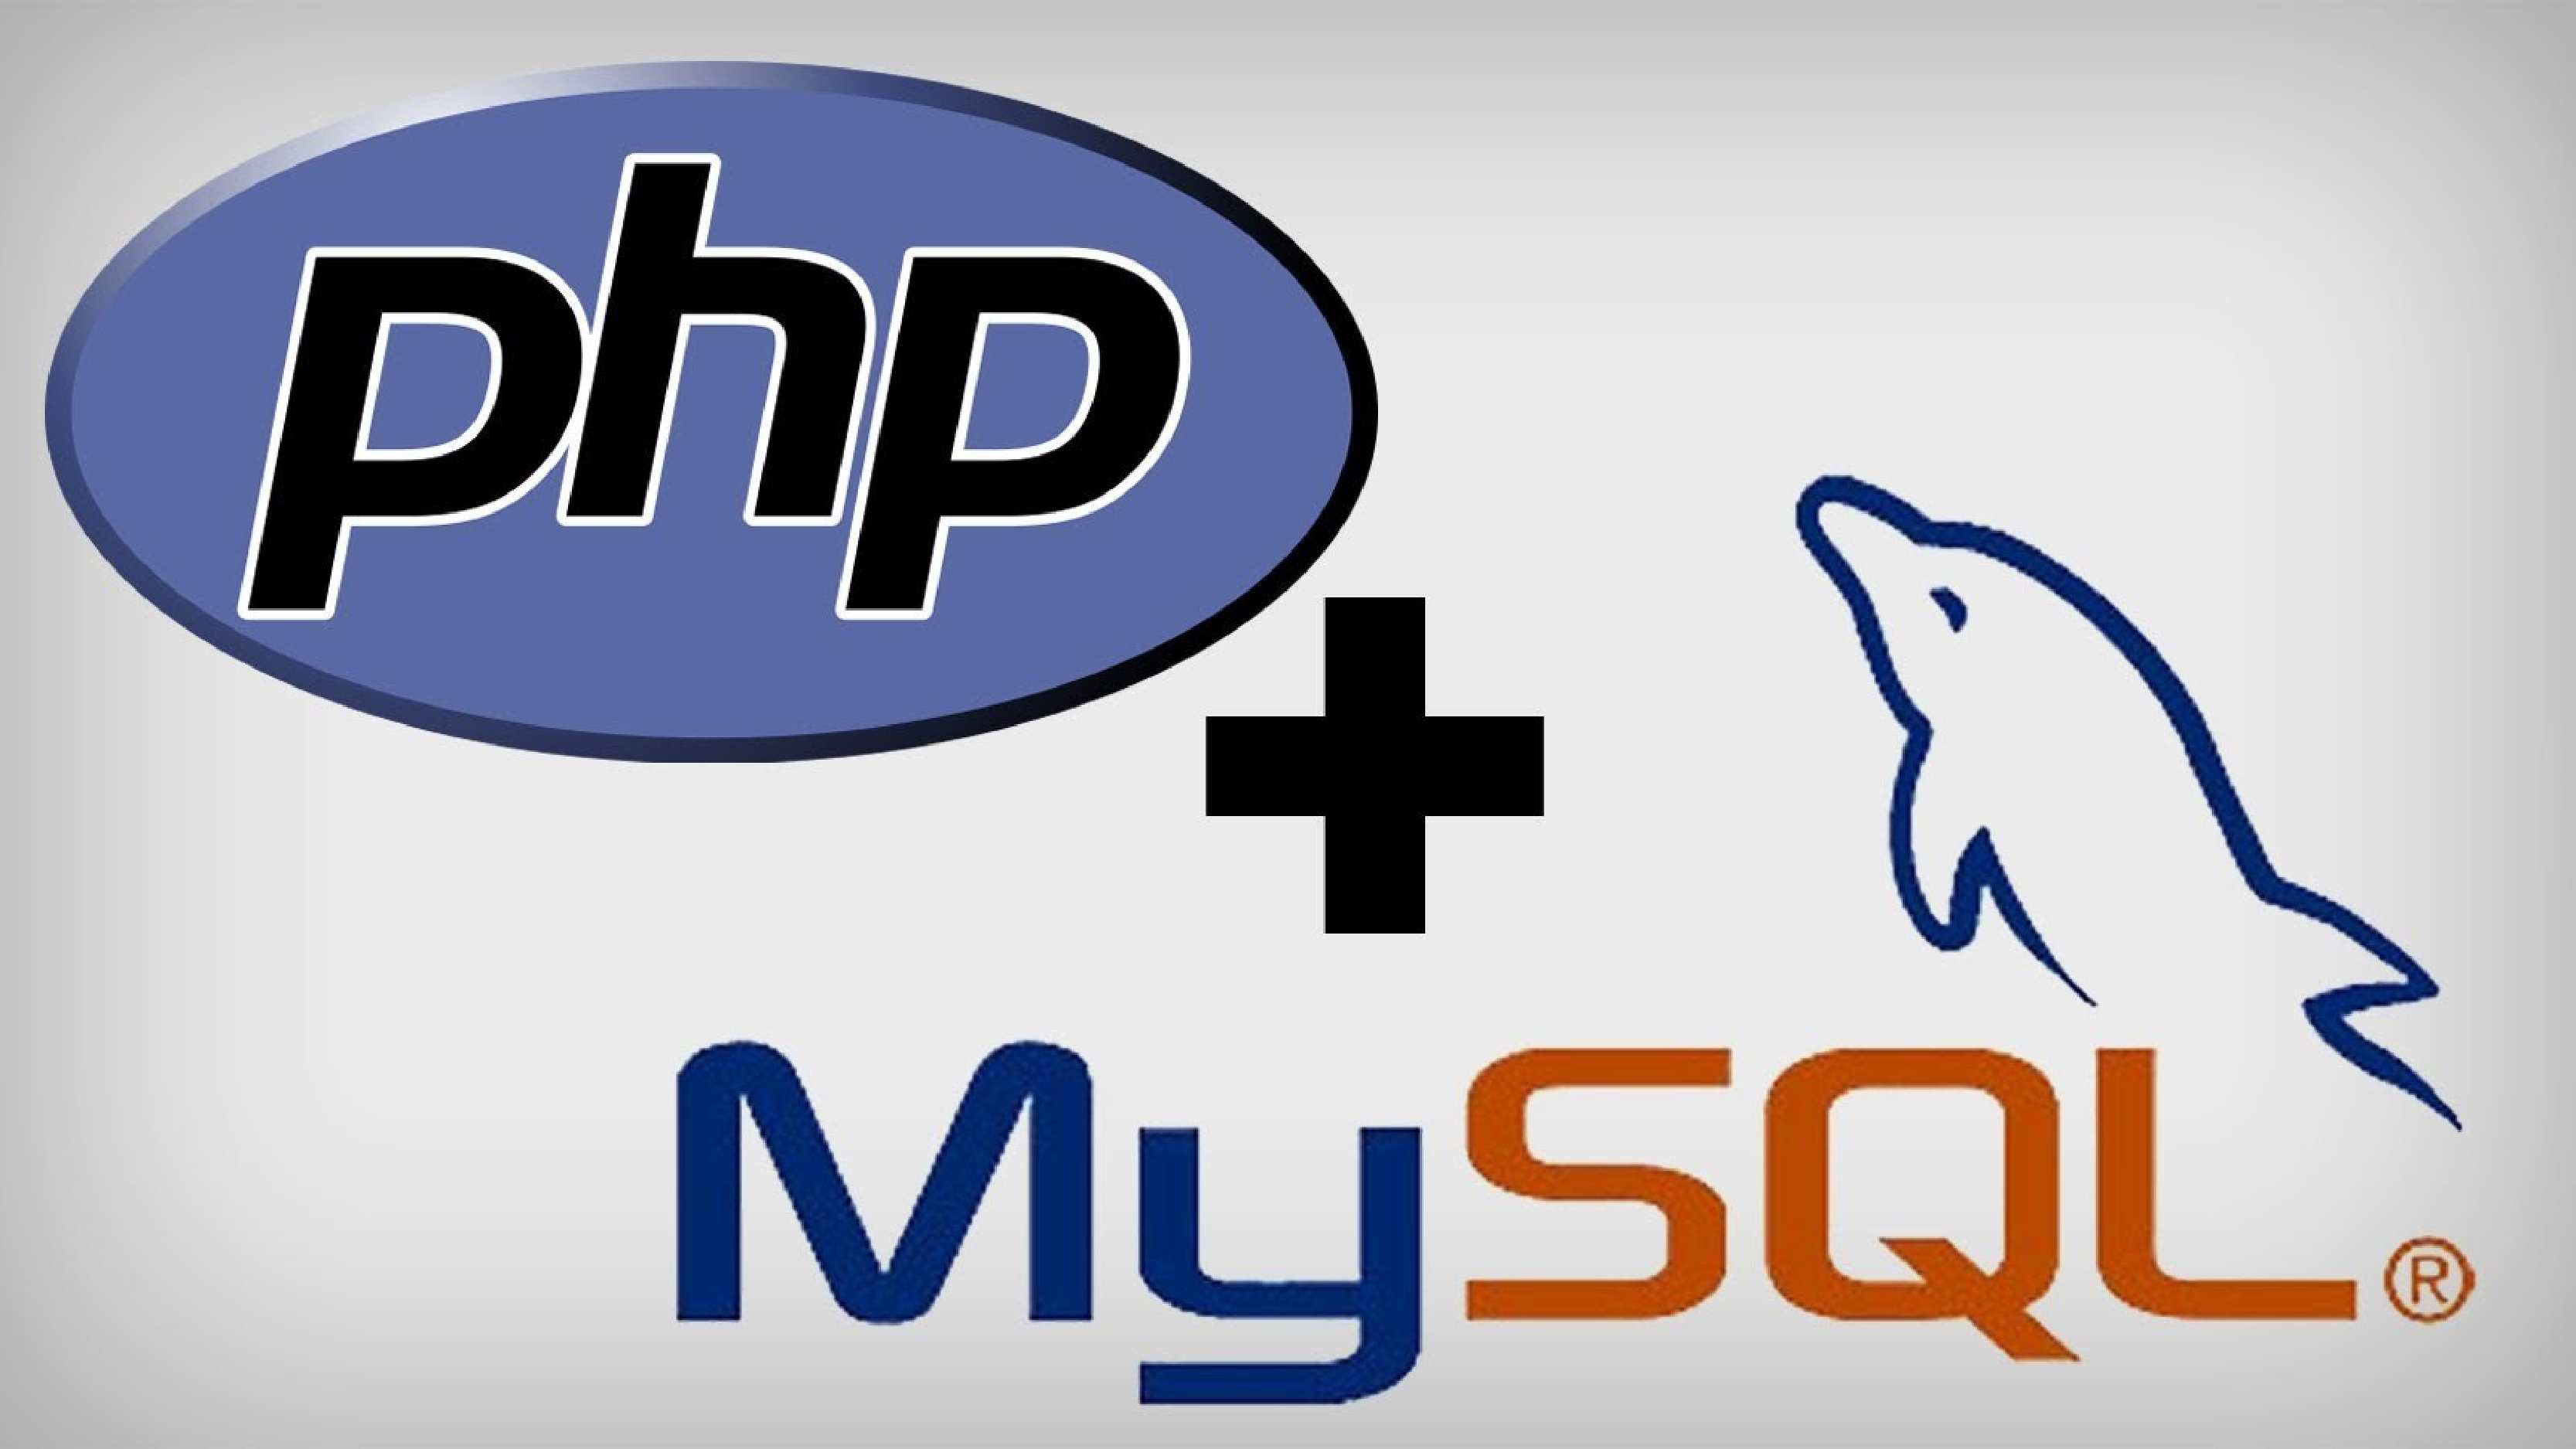
\includegraphics[width=.9\textwidth ,height=.65\textwidth]{Pic/PHP-MYSQL}
    \caption{ لوگوی 
        \lr{MySQL \&  PHP}   
    }
    \label{MYSQL-PHP}
\end{figure}
\section{ساخت یک پیشخوان}
پیشنهاد می‌شود، فایل پی‌اچ‌پی پیشخوان را در شاخه اصلی سرور یعنی همان پوشه به اشتراک گزاری شده که در قسمت‌های قبل آموزش دادیم، ذخیره کنید. سپس پوشه‌های دیگری را درون آن و بر اساس نام پروژه یا وب‌سایت در حال توسعه ساخته و پیوند به آن پوشه‌ها را هم در داخل این پیشخوان قرار دهید. همچنین می‌توانید این فایل را در پوشه‌ای با نام پیشخوان یا سندباکس ریخته و فایل شاخص در سرور خود را با نوشتن دستوراتی به این فایل انتقال دهید.

در فرآیند ساخت و ایجاد این فایل نیاز به  نصب برخی ابزار و نرم‌افزارها مانند پی‌اچ‌پی مای‌ادمین خواهید داشت، که نصب این ابزار و نرم‌افزارها برای اجرای این فایل کمک بزرگی خواهند بود. این فایل از یک بانک اطلاعاتی استفاده می‌کند که تمامی پیوندها به همراه اطلاعات مورد نیازشان در آن ذخیره شده‌است و برای درج موارد جدید به پیشخوان تنها کافی است بانک اطلاعاتی مرتبط با پیشخوان را ویرایش کرده و موارد دلخواه را به آن افزوده یا حذف کنید.
\section{نصب پی‌اچ‌پی مای‌ادمین
     \lr{«PHPMyAdmin»}
     }
پی‌اچ‌پی مای‌ادمین یک نرم‌افزار مبتنی بر وب متن‌باز / آزاد است که در سیستم‌عامل گنو/لینوکس و اکثر توزیع‌های مطرح به راحتی قابل نصب است. نحوه کار این نرم‌افزار به شکلی است که اگر آدرس سرور را به همراه عبارت پی‌اچ‌پی مای‌ادمین «phpmyadmin» بنویسید، وارد صفحه‌ای خواهید شد که با نوشتن نام کاربری و رمز عبور مای‌اس‌کیوال به شما اجازه ساخت و ویرایش جداول و … را می‌دهد. همچنین ابن ابزار علاوه بر امکان حذف و ویرایش و مدیریت گرافیکی مای‌اس‌کیوال، نرم‌افزار خوبی برای رفع ایراد و مشکلات بانک‌های اطلاعاتی و کدهای نوشته شده برای دسترسی و ویرایش اطلاعات هستند. به شکلی که با دسترسی به این ابزار می‌توان مشکلات احتمالی در کدهای نوشته شده و حتی بانک اطلاعاتی را به شکلی ساده مشاهده کنید.

در ابزار تحت وب پی‌اچ‌پی مای‌ادمین به‌علاوه اینکه دسترسی گرافیکی و ساده‌ای را برای ویرایش، ایجاد و حذف اطلاعت و جداول در اختیار دارید، همواره خواهید توانست با استفاده از نوشتن دستورات و پرس‌وجوی اس‌کیوال، اطلاعات و بانک اطلاعاتی خود را ویرایش و تغییر دهید. برای نصب این ابزار، ابتدا ماشین مجازی سندباکس را اجرا کنید و بعد از اینکه سیستم‌عامل گنو/لینوکس توزیع اوبونتو (عبارت سیستم‌عامل اوبونتو صحیح نیست) به طور کامل اجرا شد، دستور زیر را برای اتصال به آن اجرا کنید. (جهت یادآوری)
\begin{figure}
    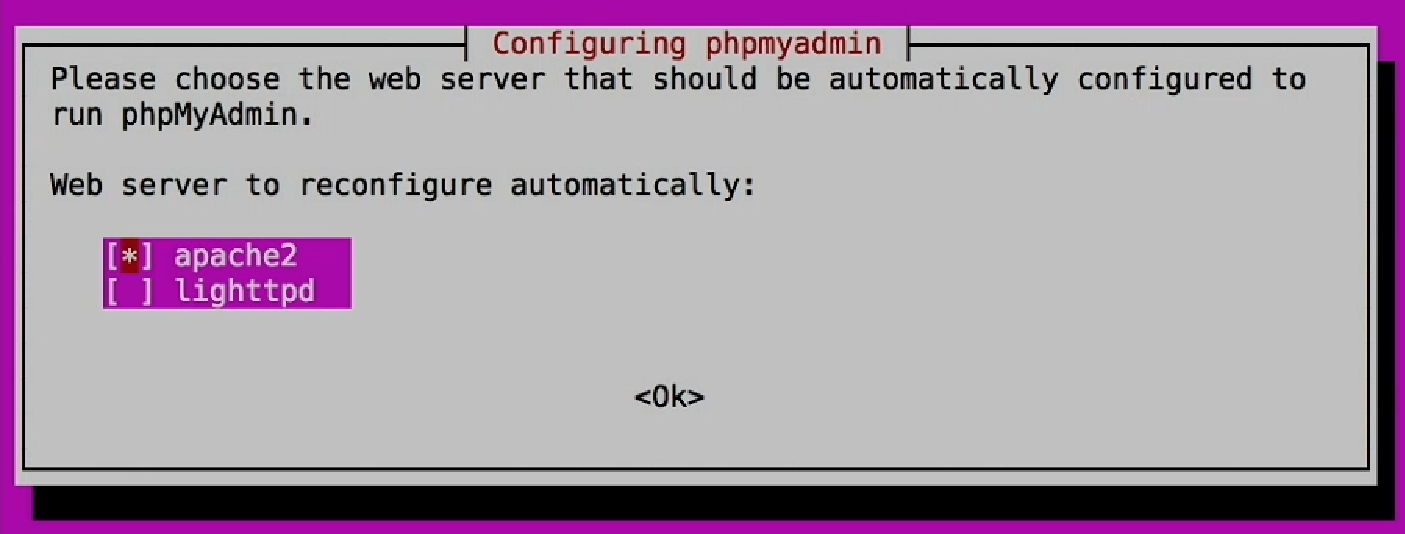
\includegraphics[width=.9\textwidth ,height=.35\textwidth]{Pic/PHPADMIN}
    \caption{ تنظیمات 
        \lr{PHPMyAdmin}   
    }
    \label{PHPMyAdmin}
\end{figure}


\begin{latin}  
    \lstinputlisting[numbers=right,language=Bash, framexleftmargin=5mm, frame=shadowbox,rulesepcolor=\color{Black}]{Code/pmyadmin1.sh}
\end{latin}

بعد از ورود به  توزیع اوبونتو نگارش سرور و نمایش اعلان سیستم، دستور زیر را اجرا کنید تا بسته‌نرم‌افزاری مورد نظر از طریق ابزار متنی ای‌پی‌تی «APT» نصب شود.
\begin{latin}  
    \lstinputlisting[numbers=right,language=Bash, framexleftmargin=5mm, frame=shadowbox,rulesepcolor=\color{Black}]{Code/pmyadmin2.sh}
\end{latin}
بعد از نوشتن دستور بالا، برخی تنظیمات برای اجرای صحیح این ابزار در سیستم، نمایش داده خواهند شد. این تنظیمات را به شکل زیر تکمیل کنید. در مرحله اول بر روی آپاچی کلید فاصله «Space» را فشار داده و با زدن کلید «TAB» و فشردن بر دکمه اینتر «Enter»، وارد مرحله بعدی شوید.
\ref{PHPMyAdmin}
در این مرحله که مرتبط با ساخت یک بانک اطلاعاتی جهت ذخیره تنظیمات این نرم‌افزار است، نیز پیغام نمایش داده شده را به صورت پیش‌فرض رها کرده و فقط دکمه اینتر را فشار داده تا وارد مرحله بعدی شوید.
\ref{PHPMyAdmin2}
\begin{figure}
    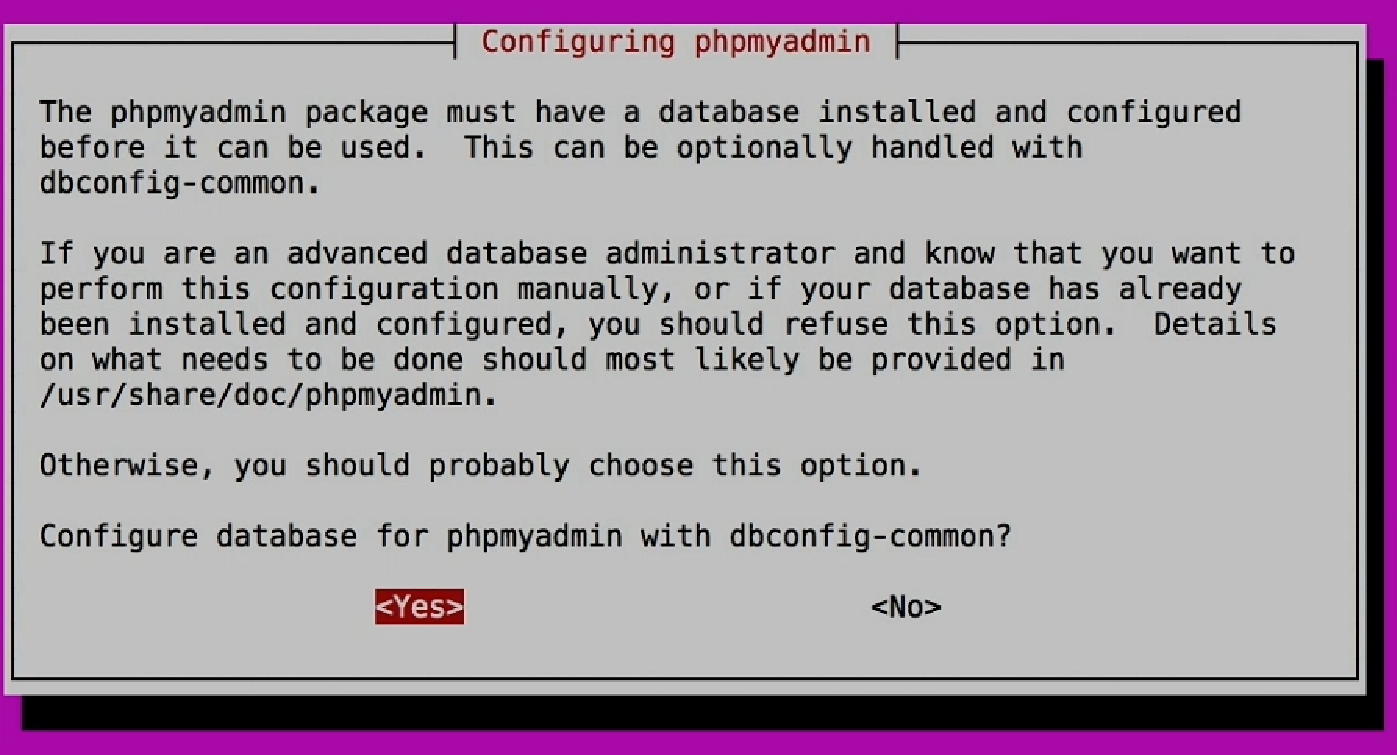
\includegraphics[width=.9\textwidth ,height=.45\textwidth]{Pic/PHPADMIN2}
    \caption{ تنظیمات 
        \lr{PHPMyAdmin .Figure-2)}   
    }
    \label{PHPMyAdmin2}
\end{figure}

در کادر نمایش داده شده، گذرواژه کاربر ریشه و مدیر مای‌اس‌کیوال را وارد کنید و سپس با فشردن کلید اینتر وارد مرحله بعدی شوید. در کادر به نمایش درآمده داخل پیغام بعدی نیز، باید گذرواژه کاربر مدیر را وارد کنید، این کار باعث دسترسی به تمامی بانک‌ها و کاربران خواهد بود. در این مرحله با خالی گذاشتن گذرواژه، کلید  
\path{«TAB»}
را فشار داده و بر روی گزینه تایید 
\path{«OK»}
 کلید اینتر  
\path{«Enter»}
  از صفحه‌کلید را فشار دهید. در اینجا ما برای نام کاربری مدیر «admin» در ابزار پی‌اچ‌پی مای‌ادمین از گذرواژه استفاده نکرده‌ایم اما برای مای‌اس‌کیوال از گذرواژه «root» با حروف کوچک استفاده کرده‌ایم. در مجموع در این مرحله که کادری مشابه کادر زیر است، گذرواژه را وارد خواهید کرد که ما آن را به شکل خالی رها کرده و تایید می‌کنیم. این کار در یک سندباکس به صورت محلی و برای راحتی کار در هر بار دسترسی به نرم‌افزار پی‌اچ‌پی مای‌ادمین گزینه معقولی است، اما برای استفاده و کاربرد تجاری، گذرواژه‌ها باید ترکیبات پیچیده‌ای از حروف و ارقام باشند.
  \ref{PHPMyAdmin3}
\begin{figure}
      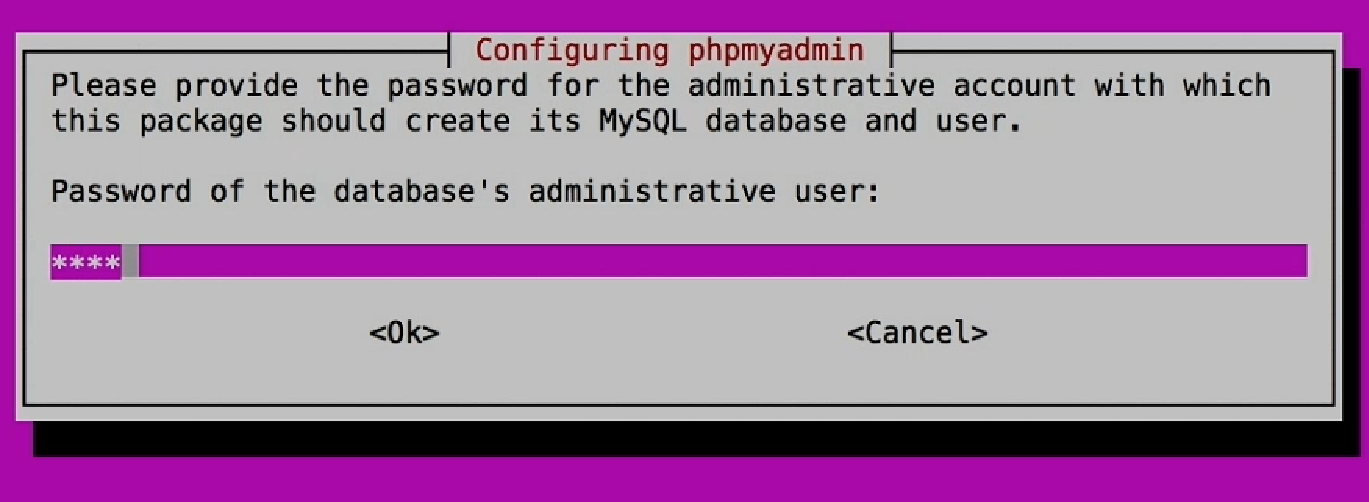
\includegraphics[width=.9\textwidth ,height=.35\textwidth]{Pic/PHPADMIN3}
      \caption{ تنظیمات 
          \lr{PHPMyAdmin .Figure-3)}   
        }
        \label{PHPMyAdmin3}
\end{figure}
مجددا عرض می‌کنم که تنظیمات بالا هرگز برای یک محیط تجاری و یک سرور واقعی مناسب نیستند، اما برای یک سندباکس و سرور محلی تنظیمات خوبی هستند. بعد از آنکه این تنظیمات با موفقیت به پایان رسید، دستور زیر را در خط فرمان اجرا کنید تا برخی تنظیمات آن را به شکل دستی انجام دهیم.
\begin{latin}  
    \lstinputlisting[numbers=right,language=Bash, framexleftmargin=5mm, frame=shadowbox,rulesepcolor=\color{Black}]{Code/pmyadmin3.sh}
\end{latin}
سپس زمانی که ویرایشگر نانو باز شد، با کلید‌های 
\path{CTRL + W}
 به دنبال عبارت «Authentication Type» بگردید. در خطوط یافت شده عبارت «cookie» را به «config» تغییر دهید. (مشابه شکل \ref{PHPMyAdmin4})

\begin{figure}
    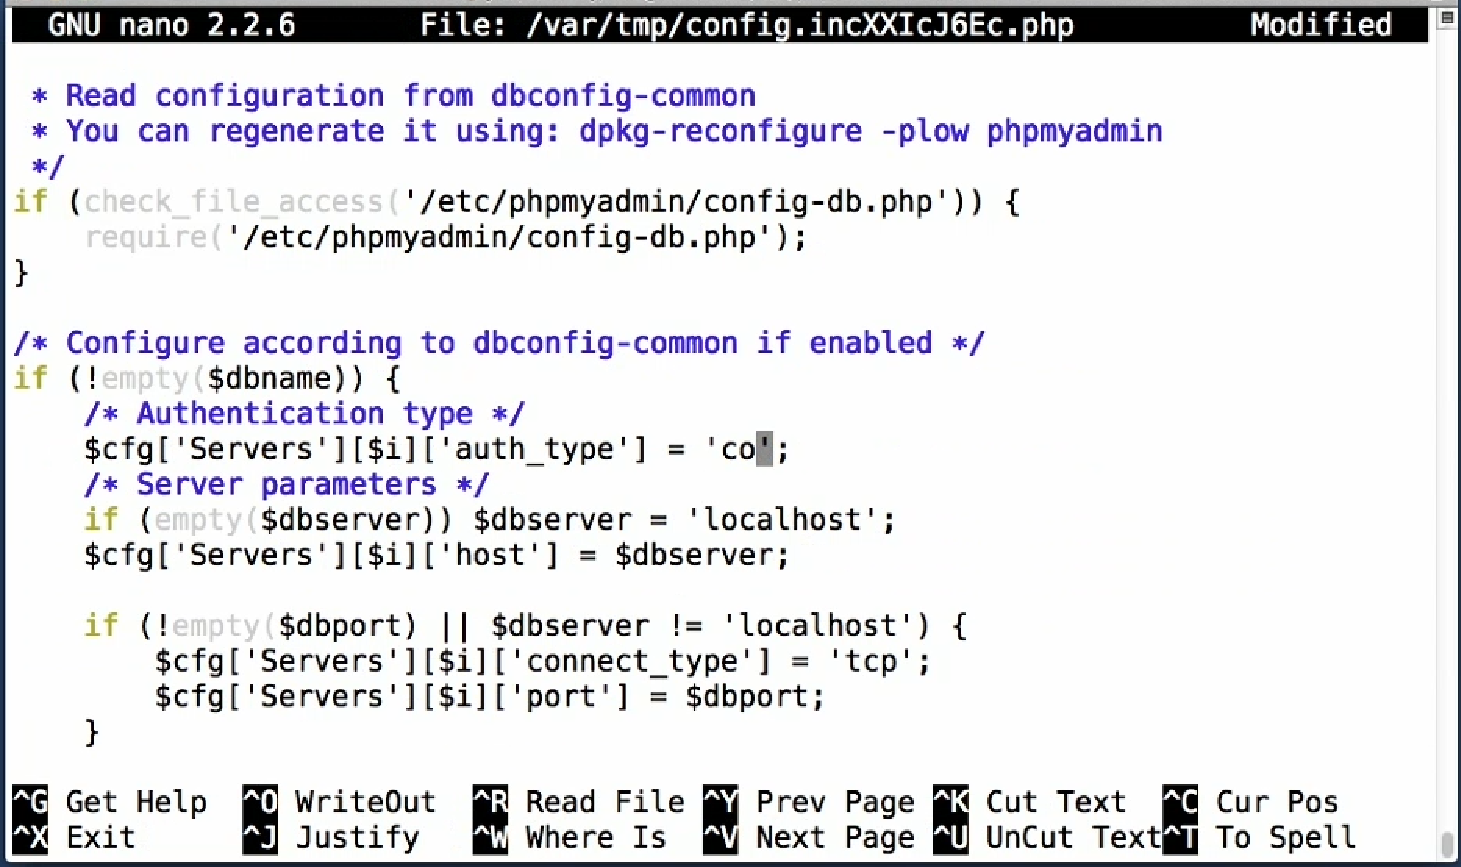
\includegraphics[width=.9\textwidth ,height=.55\textwidth]{Pic/PHPADMIN4}
    \caption{ تنظیمات 
        \lr{PHPMyAdmin .Figure-4)}   
    }
    \label{PHPMyAdmin4}
\end{figure}
سپس در همان خطی که هستید، از کلید‌های 
\path{«CTRL + K»}
 برای برش آن خط استفاده کنید و با استفاده از کلیدهای 
 \path{«CTRL + U»}
 ، کدها را سه مرتبه مجددا درج‌کنید تا مانند تصویر سه خط مشابه هم در تنظیمات ایجاد شود.
 \ref{PHP-MyAdmin2}
\begin{figure}
    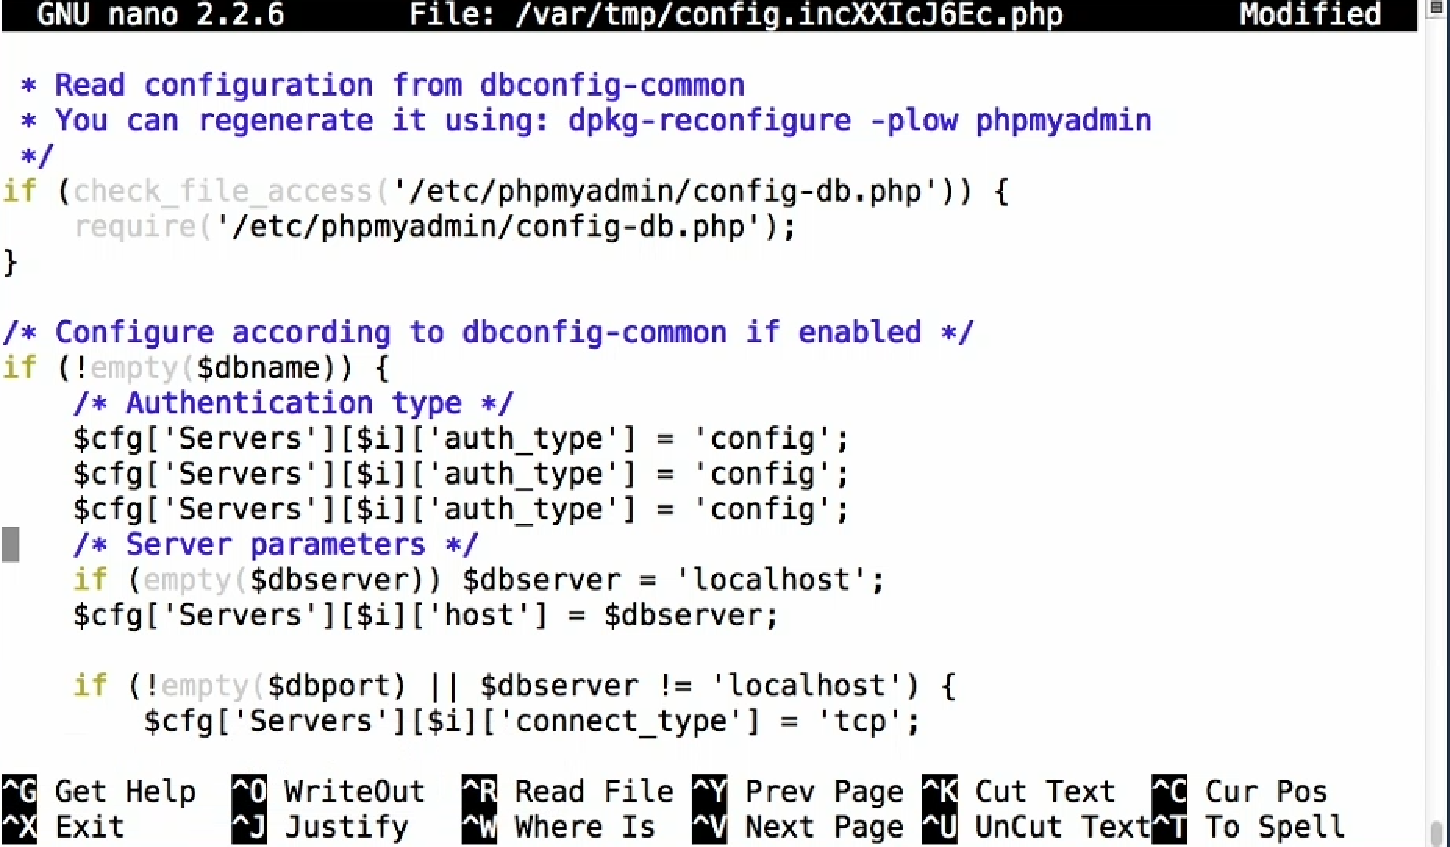
\includegraphics[width=.9\textwidth ,height=.55\textwidth]{Pic/PHPADMIN5}
    \caption{ تنظیمات 
        \lr{PHPMyAdmin .Figure-5)}   
    }
    \label{PHP-MyAdmin2}
\end{figure}
خطوط دوم و سوم را نیز به خطوط زیر تغییر دهید. برای این‌کار باید موارد مذکور را کمی تغییر دهید.
\begin{latin}  
    \lstinputlisting[numbers=right,language=Bash, framexleftmargin=5mm, frame=shadowbox,rulesepcolor=\color{Black}]{Code/pmyadmin2.sh}
\end{latin}
بعد از ذخیره فایل بالا، تنظیمات پی‌اچ‌پی مای‌ادمین تقریبا به پایان رسیده‌است. تنظیمات آخر برای تنظیم ابزار بالا برای دسترسی بدون نوشتن نام‌کاربری و گذرواژه انجام شد که باعث دسترسی سریع‌تر به ابزار بالا می‌شود. مجددا تذکر می‌دهم که این تنظیم را در یک سرور واقعی انجام ندهید. بعد از آنکه آدرس زیر را در مرورگر وارد کنید با صفحه تصویر 
\ref{PHPMyAdmin5}
 مواجه خواهید شد.
 
 \begin{figure}
     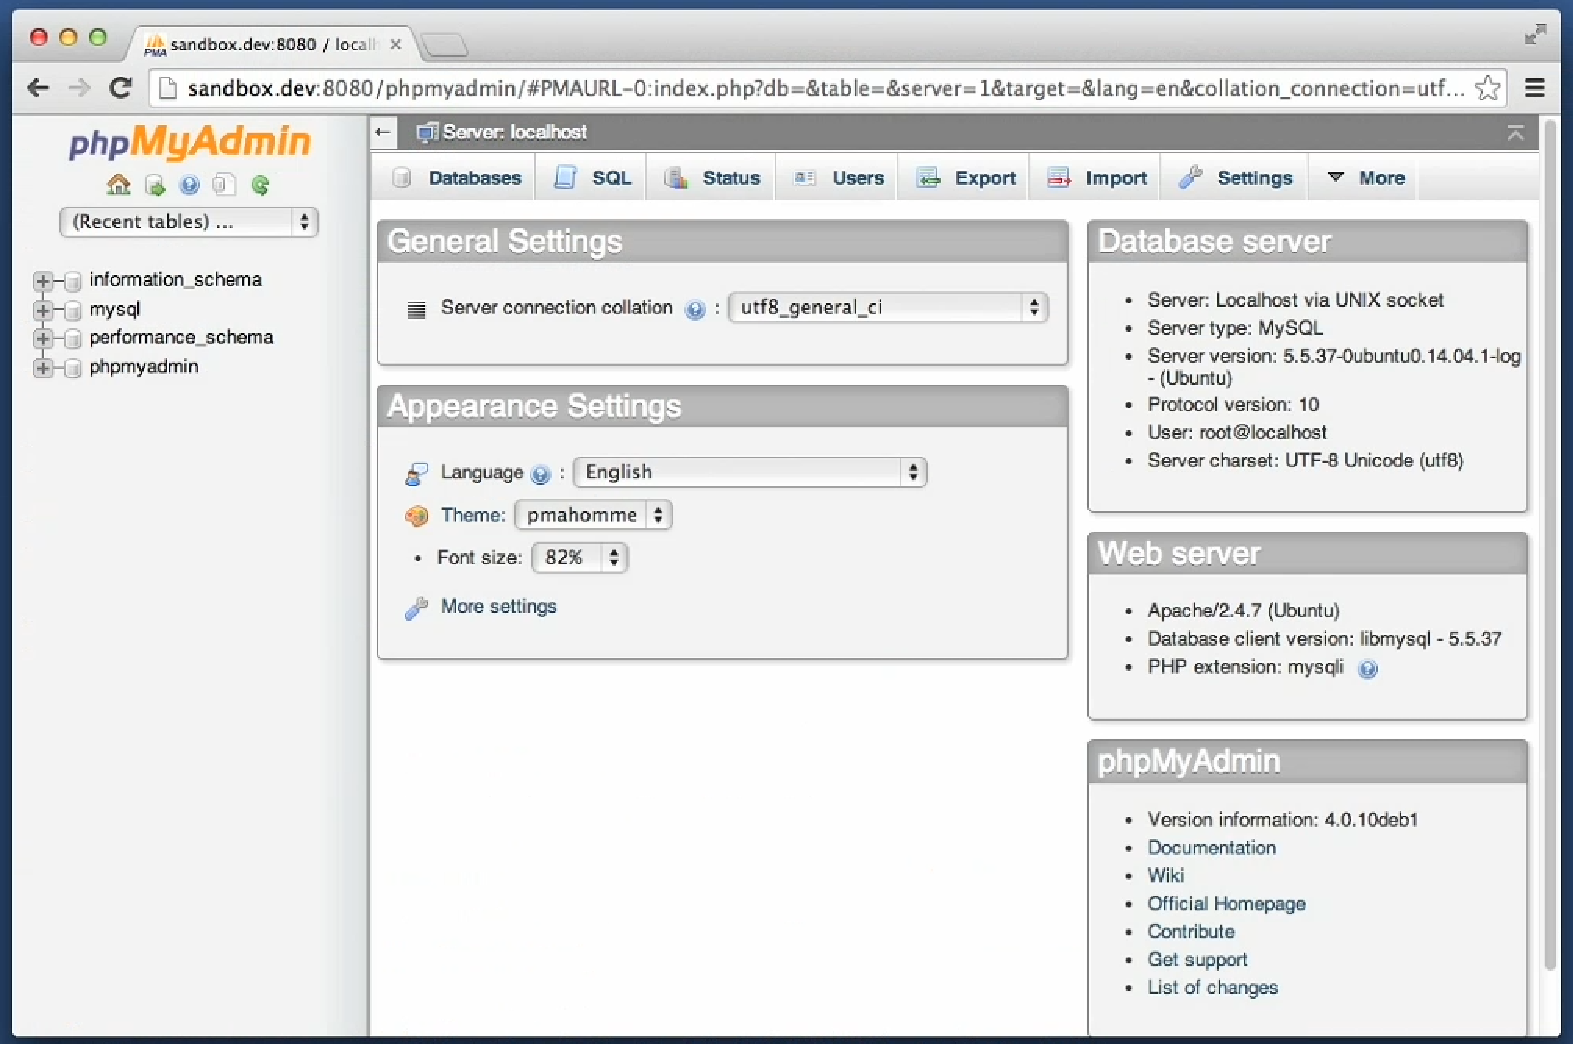
\includegraphics[width=.9\textwidth ,height=.65\textwidth]{Pic/PHPMYADMIN-UI}
     \caption{ صفحهٔ اصلی نرمافزار  
         \lr{PHPMyAdmin | Home-Page)}   
        }
        \label{PHPMyAdmin5}
    \end{figure}
    بعد از آنکه صفحه‌ای مشابه با تصویر بالا را مشاهده کردید و خطای خاصی مشاهده نشد. باید دو بانک اطلاعاتی را توسط پی‌اچ‌پی مای‌ادمین ایجاد کنیم که برای کارهای بعدی مورد نیازمان خواهد بود. اولین بانک اطلاعاتی، بانک اطلاعاتی پیشخوان است و دومین بانک اطلاعاتی را برای قرار دادن جداول مورد نیاز خود خواهیم ساخت. در ابتدا بیایید با نوشتن یک کوئری اس‌کیوال، لیستی از تمامی کاربران در مای‌اس‌کیوال را مشاهده نماییم. برای این کار در نرم‌افزار پی‌اچ‌پی مای‌ادمین و از گزینه‌های بالای صفحه بر روی پیوند «SQL» کلیک کنید. در کادر نمایش داده شده، دستورات زیر را وارد کنید. برای از بین بردن دستورات موجود در این کادر بر روی دکمه «Clear» کلیک کنید تا کادر کاملا خالی شود، سپس فرامین زیر را بنویسید.
    
\begin{latin}  
    \lstinputlisting[numbers=right,language=SQL, framexleftmargin=5mm, frame=shadowbox,rulesepcolor=\color{Green}]{Code/select-user.sql}
\end{latin}

بعد از اجرای دستور بالا و کلیک بر روی دکمه رفتن «Go» لیستی از کاربران موجود در مای‌اس‌کیوال نمایش داده خواهد شد. تصویر \ref{GO-USERS}
 \begin{figure}
     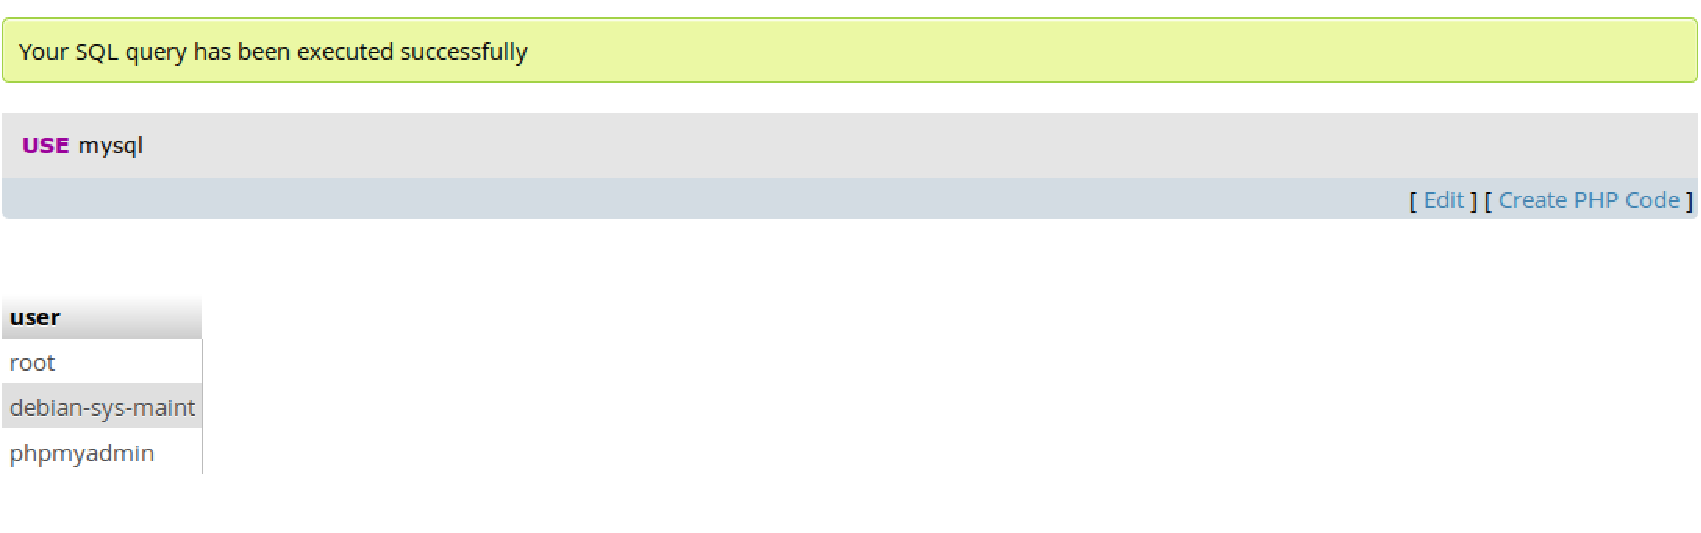
\includegraphics[width=.9\textwidth ,height=.35\textwidth]{Pic/SQL-USER-GO}
     \caption{ بر روی دکمه GO کلیک کنید 
         \lr{PHPMyAdmin)}   
        }
        \label{GO-USERS}
    \end{figure}

\section{ساخت جداول و کاربران مورد نیاز در سندباکس}
حال که نرم‌افزار پی‌اچ‌پی مای‌ادمین برای ایجاد بانک اطلاعاتی را در اوبونتو سرور نصب کردید، باید از طریق پی‌اچ‌پی مای‌ادمین دو کاربر جدید و دو بانک اطلاعاتی همنام با پایگاه‌های داده ایجاد شده را ایجاد کنیم. (بانک اطلاعاتی و پایگاه داده تقریبا به مفهوم مشابهی اشاره دارند.) این دو بانک اطلاعاتی همانطور که ذکر شد، با نام‌های پیشخوان و سندباکس برای نگاهداری اطلاعات و مقادیر پیشخوان و دیگر موارد مورد نیاز در ادامه آموزش ساخته می شوند. هر یک از این بانک‌ها توسط کاربر همنام خود قابل تغییر و دستیابی هستند که برای سهولت استفاده از گذرواژه یکسان با نامشان برخوردار خواهند بود. البته می‌توانید از گذرواژه دلخواه خود نیز بهره گیرید. برای ساخت کاربر اول از طریق صفحه «Query» با پرس‌وجوهایی که در آن توانستیم لیستی از کاربران را مشاهده کنیم، دستورات زیر را اجرا کرده و با دستور زیر یک کاربر با نام سندباکس ایجاد می‌کنیم بعد از این کار یک بانک‌اطلاعاتی همنام را نیز ایجاد می‌کنیم که کاربر بالا تنها قادر به دسترسی به این بانک اطلاعاتی خواهد بود.
\newline
\begin{latin}  
    \lstinputlisting[numbers=right,language=SQL, framexleftmargin=5mm, frame=shadowbox,rulesepcolor=\color{Green}]{Code/new-sandbox-user.sql}
\end{latin}

برای ایجاد کاربر پیشخوان از دستورات مشابه با دستور بالا استفاده خواهیم کرد. در این موقع هر آنچه با عبارت سندباکس وجود دارد را به عبارت پیشخوان تغییر می‌دهیم. با استفاده از پی‌اچ‌پی مای‌ادمین و به صورت گرافیکی نیز می‌توان تمامی مواردی که به صورت کوئری اس‌کیوال نوشته شده‌است را انجام داد. با وجود اینکه آموزش گرافیکی در یک مطلب آموزشی، بسیار دشوارتر است، از کدهای آن استفاده کرده‌ایم. اما در صورت دلخواه خود می‌توانید از ابزارهای گرافیکی مانند مای‌اس‌کیوال ورک‌‌برنچ یا پی‌اچ‌پی مای‌ادمین نیز استفاده کنید.
\newline

\begin{latin}  
    \lstinputlisting[numbers=right,language=SQL, framexleftmargin=5mm, frame=shadowbox,rulesepcolor=\color{Green}]{Code/new-dash-user.sql}
\end{latin}

لازم به ذکر است بعد از ایجاد و حذف کاربر یا تغییرات در کاربران باید  یک‌بار مجددا تمامی مجوزها از نوع به‌روز شوند. برای به‌روز کردن مجدد مجوزها از دستور زیر استفاده کنید.
\newline

\begin{latin}  
    \lstinputlisting[numbers=right,language=SQL, framexleftmargin=5mm, frame=shadowbox,rulesepcolor=\color{Green}]{Code/flush-pri.sql}
\end{latin}

بعد از آنکه کاربران بالا با موفقیت به مای‌اس‌کیوال افزوده شدند، می‌توانید از طریق پیشخوان، پیوندهای مورد نیاز به بخش‌های مختلف سرور را با ساخت یک جدول و درج مقادیر مورد نیاز انجام دهید. ابتدا ما در بانک‌اطلاعاتی پیشخوان یک جدول ساخته و مقادیر دلخواه را در آن وارد می‌کنیم. برای ساخت جدول نیز از طریق همان بخش کوئری، دستورات زیر را وارد کنید تا جدول بالا ساخته شود.
\newline

\begin{latin}  
    \lstinputlisting[numbers=right,language=SQL, framexleftmargin=5mm, frame=shadowbox,rulesepcolor=\color{Green}]{Code/create-dash-table.sql}
\end{latin}

بعد از ساخت جدول، با استفاده از پی‌اچ‌پی مای‌ادمین یا ابزار دیگر قادر خواهید بود مقادیری را به آن بیفزایید. با این حال به دلیلی که ذکر شد در این آموزش از دستورات اس‌کیوال استفاده خواهیم کرد. پس برای افزودن مقادیر جدید در یک جدول از یک بانک اطلاعاتی از دستورات اس‌کیوال استفاده خواهیم کرد. به عنوان نمونه  با دستور زیر فایل «phpinfo» واقع در آدرس مشخص شده را به پایگاه داده می‌افزاییم. این کار باعث می‌شود که آدرس و برچسبی برای این صفحه در پیشخوان ساخته شود و بعدا اگر کدی برای این بانک اطلاعاتی نوشته شد، با کلیک بر روی پیوندی با عنوان برچسب و آدرس مشخص شده به آن آدرس مراجعه کنیم که در این‌جا برچسب و آدرس برای صفحه اطلاعات پی‌اچ‌پی است که در قسمت قبل آن را ایجاد کرده‌ایم.
\newpage


\begin{latin}  
    \lstinputlisting[numbers=right,language=SQL, framexleftmargin=5mm, frame=shadowbox,rulesepcolor=\color{Green}]{Code/insert-into-dash-table.sql}
\end{latin}

همانطور که ذکر شد، تمامی اعمال بالا را می‌توان توسط پی‌اچ‌پی مای‌ادمین و به صورت گرافیکی انجام داد. با این حال همواره می‌توانید کد بالا را برای هر بار افزودن پیوند جدید اجرا کنید. یا اینکه  با استفاده از پی‌اچ‌پی صفحه‌ای را برای درج مقادیر جدید بنویسید که بسته به سلیقه خود می‌توانید یکی از این کارها را انجام دهید.نوشتن یک صفحه جدید برای افزودن مقادیر به پیشخوان کار تقریبا ساده‌ای است و با نوشتن یک فایل پی‌اچ‌پی ساده که دستور اس‌کیوال بالا را اجرا می‌کند، خواهید توانست چنین صفحه‌ای را ایجاد کنید. یکی از دلایلی که در این آموزش به جای راه حال گرافیکی از دستورات اس‌کیوال استفاده شده است نیز همین مورد است. در این آموزش شما می‌توانید با استفاده از دستورات اس‌کیوال نوشته شده صفحات و یا اسکریپت دلخواه خود را برای انجام کارهای تکراری بنویسید.
\section{فایل پیشخوان}
پیوندهایی که باید در داخل فایل پیشخوان نمایش داده شوند در داخل بانک اطلاعاتی با همین نام ذخیره شده‌است، برای استفاده از این بانک اطلاعاتی و مقادیر و مسیرهای وارد شده در آن می‌توان از زبان برنامه‌نویسی پی‌اچ‌پی استفاده کرد و با نوشتن یک فایل، مقادیر موجود در یک جدول را نمایش داد. برای این کار من یک فایل پی‌اچ‌پی را از قبل آماده کرده‌ام که آن را در پوشه «dashboard» ذخیره می‌کنید. سپس بعد از ذخیره فایل بالا در آن پوشه فایل دیگری را نیز با نام فایل شاخص «index.php» در شاخه اصلی می‌ریزیم. کد فایل پیشخوان به صورت زیر است. در این حالت کدهای زیر را در شاخه «dashboard» و با نام «index.php» ذخیره کنید. این کار باعث ایجاد صفحه پیشخوانی مشاهده می‌شود که دارای ساختاری ساده است. همانطور که گفته شد، در این مطلب قصد آموزش زبان پی‌اچ‌پی را نداشته و فقط برای راحتی کار کدهای زیر را در اینجا قرار داده‌ام.
\newpage

\begin{latin}  
    \lstinputlisting[numbers=right,language=PHP, framexleftmargin=5mm, frame=shadowbox,rulesepcolor=\color{Blue}]{Code/dashboard.php}
\end{latin}

کدهای زیر را نیز در شاخه اصلی با نام «index.php» ذخیره کنید. این کار باعث می‌شود هرگاه کاربران به آدرس سندباکس مراجعه کنند به سمت پوشه، پیشخوان «Dashboard» هدایت شوند.
\newline

\begin{latin}  
    \lstinputlisting[numbers=right,language=PHP, framexleftmargin=5mm, frame=shadowbox,rulesepcolor=\color{Blue}]{Code/index.php}
\end{latin}

سپس اگر آدرس سندباکس 
    \url{http://sandbox.dev:8080/}
را در مرورگر وارد کنید، با صفحه‌ای مانند شکل زیر مواجه خواهید شد که شامل پیوندهایی به مسیرهای دلخواه است. پیوندهای بالا از طریق بانک اطلاعاتی ایجاد شده در مراحل قبل، به این فایل وارد شده‌اند. برای بهبود ظاهر این صفحه می‌توانید فایل سی‌اس‌اس دلخواه را ایجاد کنید و به این فایل تخصیص دهید.
\ref{DASHBOARD}
\newline
\begin{figure}
    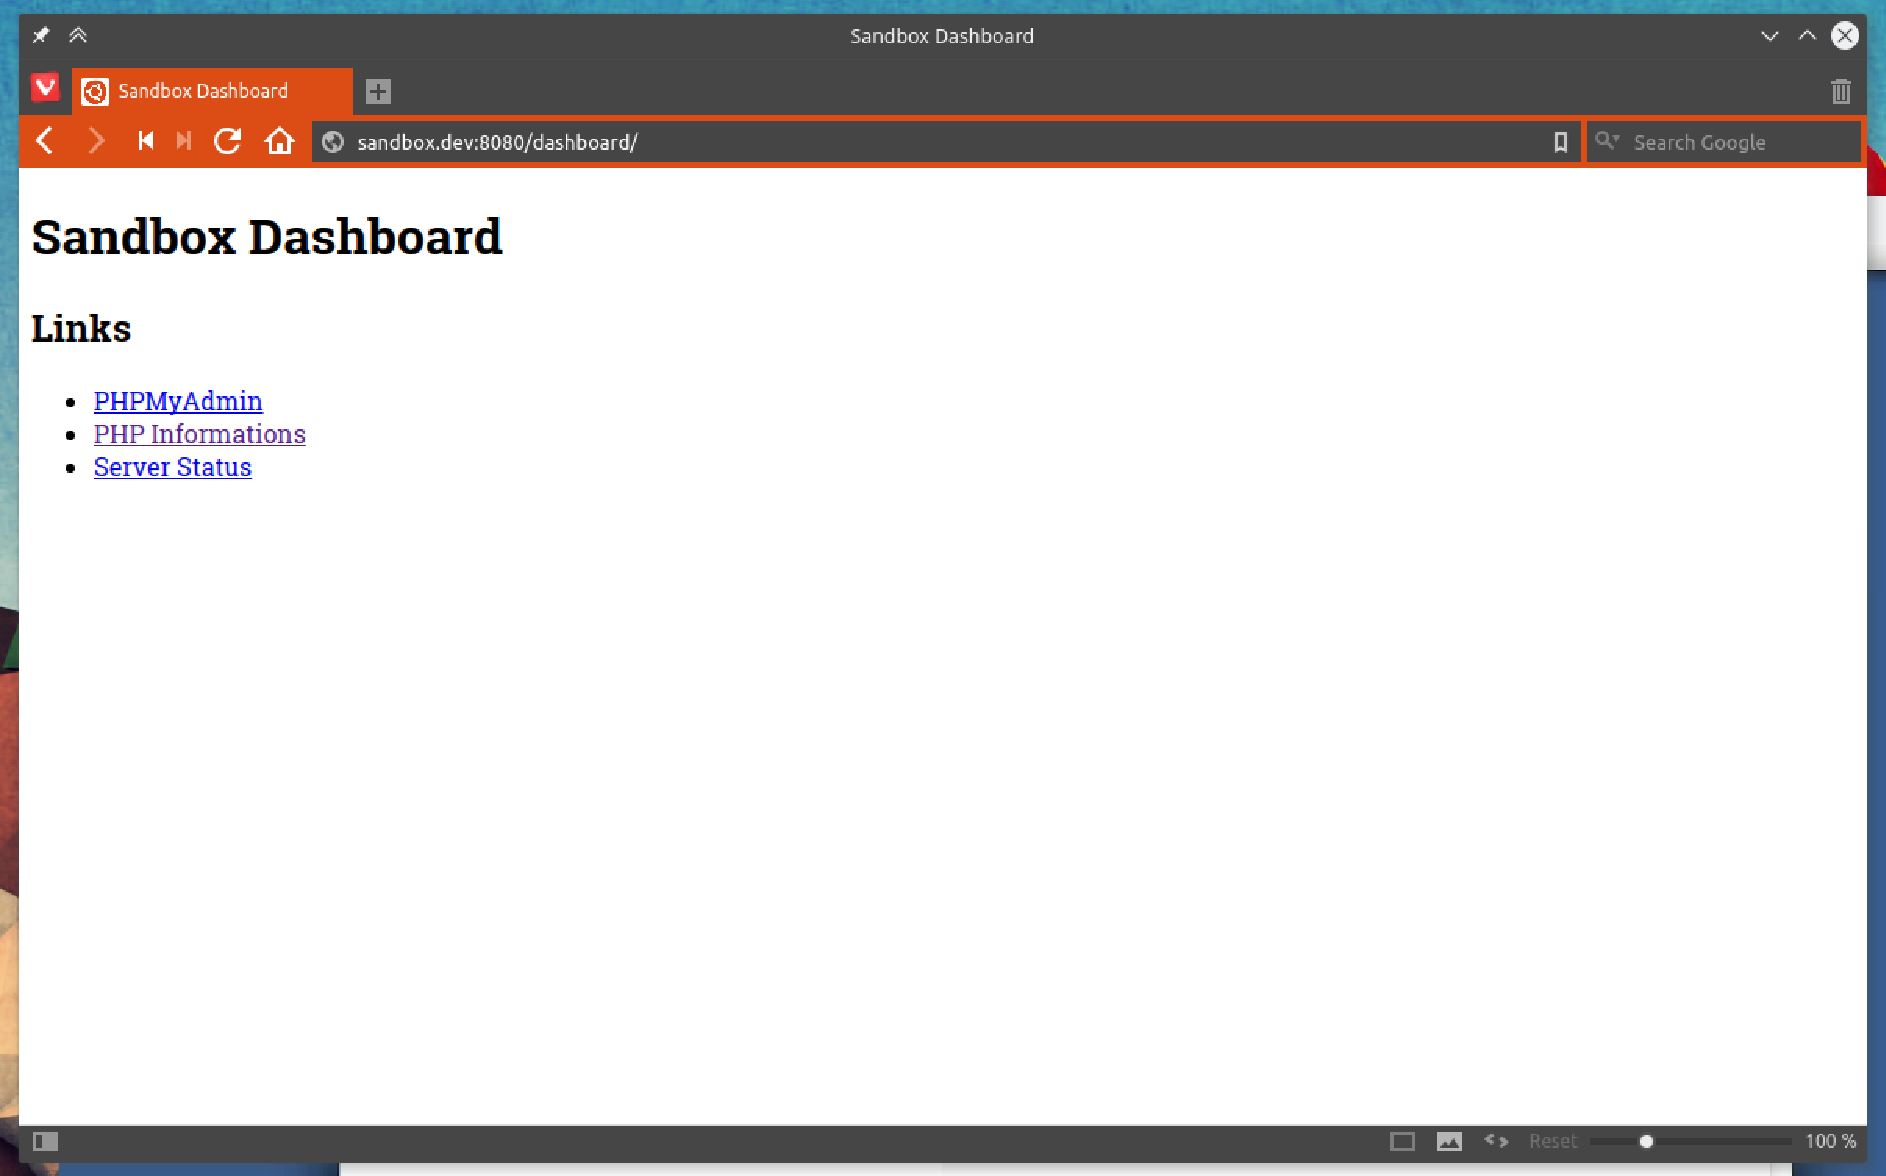
\includegraphics[width=.9\textwidth ,height=.60\textwidth]{Pic/Dashboard}
    \caption{ نمایی از داشبورد یا پیشخوان
        \lr{(Dashboard Page)}   
    }
    \label{DASHBOARD}
\end{figure}